\section{Transformación vectorial iterativa}

\begin{figure}[H]
\centering
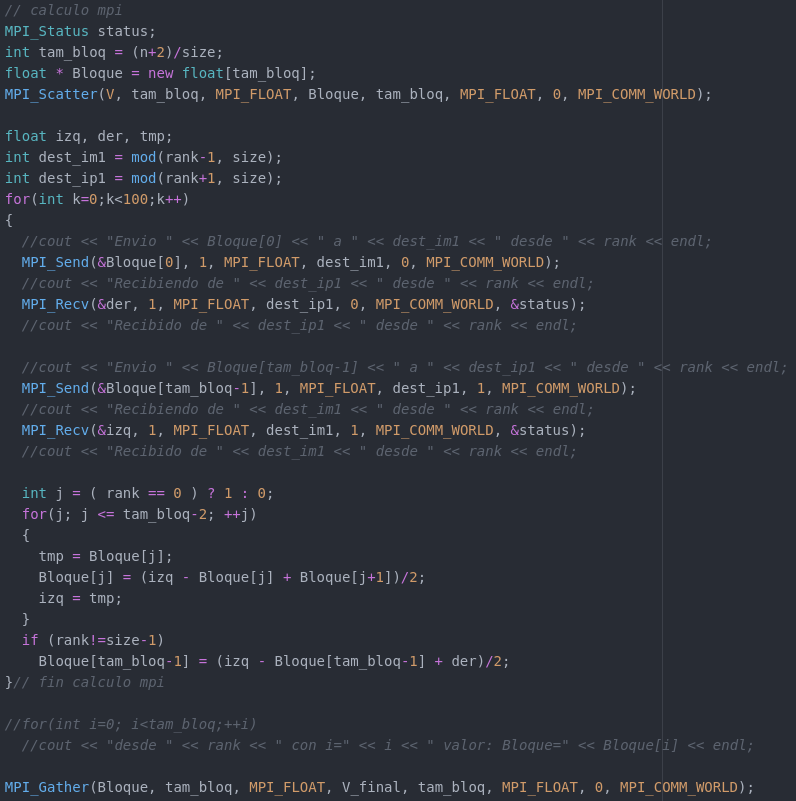
\includegraphics[width=0.8\textwidth]{imagenes/code.png}
\end{figure}

Cada proceso tiene un tamaño de bloque igual a una parte igual de $n$ más los dos extremos. Se envía casi de forma idéntica que en el pseudocódigo mostrado en las transparencias y se calcula igual excepto para los extremos: rank(0) no ejecuta la iteración 0 y rank(size-1) no ejecuta la ultima.

Finalmente se hace el gather de todos los bloques. A continuación se muestra una ejecución para n=12(10+2), en la que se pasa el mismo test que en las prácticas y se muestran todos los elementos de los vectores.

\begin{figure}[H]
\centering
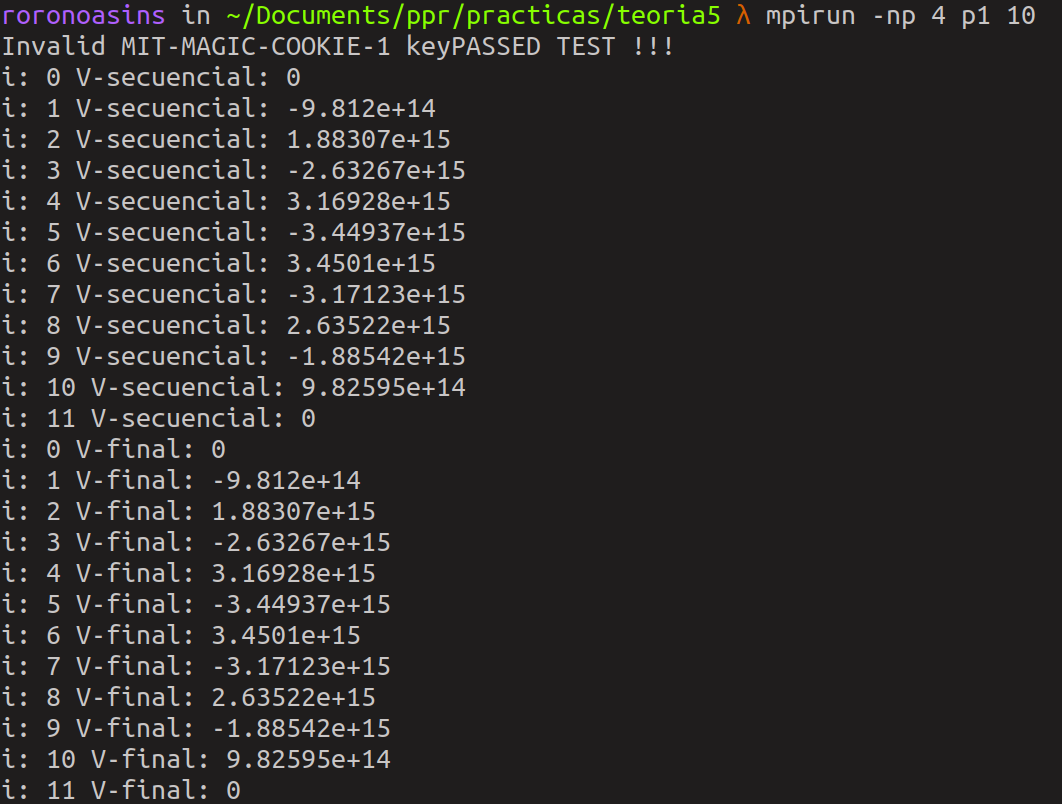
\includegraphics[width=0.8\textwidth]{imagenes/ej.png}
\end{figure}

